\documentclass[m3380-lec-main.tex]{subfiles}
\setcounter{chapter}{8}

%\DeclareMathOperator{\R}{\mathbb{R}}

\begin{document}


\chapter{Permutations}

\section*{Goals}
\begin{enumerate}[1.~]\setlength{\itemsep}{0pt}
\item Define permutations
\item Permutation operations
\item Implementation of a permutation class
\end{enumerate}

\section{What is a permutation?}
\begin{defn} Suppose $A$ is a set. Then a function $\sigma$ with domain $A$ and codomain $A$ is a \emph{permutation of $A$} if and only if $\sigma$ satisfies the following two criteria:
\begin{enumerate}[\bfseries i.]
\item (Surjective/Onto) For each element $a\in A$, there is an element $a'\in A$ such that ${\sigma(a') = a}$.
\item (Injective/One-to-one) For any elements $a,b\in A$, if $f(a)=f(b)$ then $a=b$.
\end{enumerate}
\end{defn}
Functions which are both one-to-one and onto are also called \emph{bijections}, so an easier definition of a permutation $\sigma$ of $A$ is that $\sigma$ is a bijection from $A$ to itself. It is important to note that the definition of a permutation of $A$ does not require that the set $A$ be finite. The study of permutations of infinite sets is beyond the purpose to which we will put our permutations, so we will henceforth make the following assumption: \textbf{all sets which we permute will be finite sets.}

\begin{defn} We make the following notational definitions for the sake of convenience.
\begin{itemize}
\item $\scr{E}$ is the set of letters in the English alphabet.
\item $[n] = \set{1,2,3,\ldots,n}$ whenever $n\in \mathbb{N}$.
\end{itemize}
For a finite set $A$ which is not a subset of $[n]$ for any $n$, we denote the set of all permutations of $A$ by $S_A$. The set of all permutations of $[n]$ is denoted $S_n$.
\end{defn}

\newcommand{\E}{\scr{E}}

\subsection{Representing a permutation}
There are several distinct ways of representing permutations which are useful in different situations. For non-numeric sets, one of the best is called \emph{two-line notation}.

\begin{exmp}\label{exmp:perm1}
Suppose $\sigma_1:[15]\to[15]$ is defined by $\sigma_1(i) = 16-i$. Then the \emph{two line notation} for $\sigma_1$ is
\[\begin{tlp}{\sigma_1}{15}{0/1/15, 1/2/14, 2/3/13, 3/4/12, 4/5/11, 5/6/10, 6/7/9, 7/8/8, 8/9/7, 9/10/6, 10/11/5, 11/12/4, 12/13/3, 13/14/2, 14/15/1}
\end{tlp}\]
This permutation is one which the ``best" representation is its functional one, $\sigma_1(i)=16-i$. However, this is not always the case. Consider the following permutation $\sigma_2$ of $[15]$ given by
\[\begin{tlp}{\sigma_2}{15}{0/1/4, 1/2/3, 2/3/2, 3/4/7, 4/5/6, 5/6/5, 6/7/10, 7/8/9, 8/9/8, 9/10/13, 10/11/12, 11/12/11, 12/13/1, 13/14/15, 14/15/14}
\end{tlp}\]
Worse still is this permutation $\sigma_3$ of $\E$:
\[\begin{tlp}{\sigma_3}{26}{0/a/d, 1/b/k, 2/c/b, 3/d/c, 4/e/j, 5/f/s, 6/g/m, 7/h/n, 8/i/f, 9/j/o, 10/k/a, 11/l/t, 12/m/w, 13/n/v, 14/o/z, 15/p/p, 16/q/i, 17/r/x, 18/s/u, 19/t/r, 20/u/h, 21/v/q, 22/w/y, 23/x/l, 24/y/g, 25/z/e}
\end{tlp}\]
Two line notation is especially good when there is no natural order for the symbols in the set being permuted. For example, if $A=\set{\clubsuit, \diamondsuit, \heartsuit, \spadesuit, \nabla, \surd, \infty}$, then the following is a valid permutation of $A$:
\[\begin{tlp}{\sigma_4}{7}{0/$\clubsuit$/$\diamondsuit$, 1/$\diamondsuit$/$\heartsuit$, 2/$\heartsuit$/$\spadesuit$, 3/$\spadesuit$/$\clubsuit$, 4/$\nabla$/$\surd$, 5/$\surd$/$\infty$, 6/$\infty$/$\nabla$}
\end{tlp}\]
\end{exmp}

For some sets, using both lines of the two-line notation is unnecessary. For instance, every permutation in $S_n$ has the same first row in two-line notation! For sets such as these, where there is a commonly understood order and first element, we can suppress the first line of two-line notation, and obtain \emph{one-line notation}.

\begin{exmp} We can write the permutations $\sigma_1$ and $\sigma_2$ above easily in one-line notation\footnote{There is considerable disagreement in the literature about whether the symbols in one-line notation should be separated by spaces, commas, or not at all. Anecdotally, Dr.~Kassie Archer of UT Tyler, who does research in combinatorial permutation theory, expressed that her personal preference is to use no separation if there are enough distinct elements in the set, and spaces otherwise. Our notation will follow her example.}:
\begin{align*}
\sigma_1 &= 15~14~13~12~11~10~9~8~7~6~5~4~3~2~1, \\
\sigma_2 &= 4~3~2~7~6~5~10~9~8~13~12~11~1~15~14. \\
\end{align*}
Since $\sigma_3$ is a permutation of $\E$, its one-line notation is a collection of English letters -- an unpronounceable word:
\[\sigma_3 = \text{dkbcjsmnfoatwvzpixurhqylge}.\]
Since the set $A$ defined in Example \ref{exmp:perm1} has no clear order, we cannot use one-line notation to represent $\sigma_4$.
\end{exmp}

\begin{defn} Suppose $A$ is a set, and let $e_A:A\to A$ be the function such that $e_A(a)=a$ for each $a\in A$. Then $e_A$ is the \emph{identity permutation on $A$}. When the set $A$ being permuted is clear by context, the identity permutation will simply be denoted $e$.
\end{defn}

\section{Permutation groups}
Since permutations of a set $A$ are bijections from $A$ to $A$, they can be composed.
\begin{thm}Suppose $\sigma,\tau\in S_A$ for some set $A$. Then the composition of $\tau$ after $\sigma$ is a permutation $\tau\circ\sigma:A\to A$ defined by
\[(\tau\circ\sigma)(a) = \tau(\sigma(a))\]
for each $a\in A$. Moreover, the composition symbol $\circ$ will be suppressed, and we will write $\tau\sigma$ as a product rather than a composition\footnote{This is familiar: think of $f(x) = \arctan\cos(x)$.}.
\end{thm}

Two-line notation makes calculating the composition of permutations uncomplicated, if the permutations are ``stacked" in the correct order.
\begin{exmp}
Consider $\sigma_1$ and $\sigma_2$ from Example 9.3. To determine the product $\sigma_2\sigma_1$, we write $\sigma_1$ first and then $\sigma_2$ below it, in two-line notation. The output of $\sigma_1$ then becomes the input of $\sigma_2$, as demonstrated below by an arrow.
\[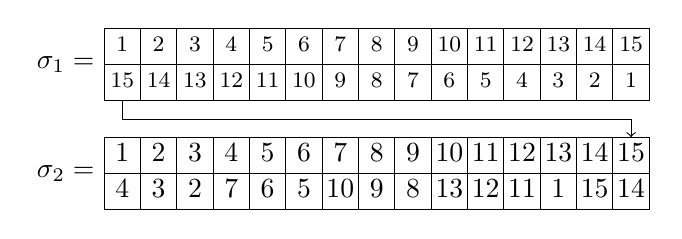
\begin{tikzpicture}[scale=12/26]
\node [left] at (0,0) {\( \sigma_1 = \)};{\footnotesize\draw[anchor=mid] (0,-1) grid (15,1) \foreach \x/\y/\z in {0/1/15, 1/2/14, 2/3/13, 3/4/12, 4/5/11, 5/6/10, 6/7/9, 7/8/8, 8/9/7, 9/10/6, 10/11/5, 11/12/4, 12/13/3, 13/14/2, 14/15/1}{(\x+1/2,1/2) node {\y} (\x+1/2,-1/2) node {\z}};}

\node [left] at (0,-3) {$\sigma_2 =$};
{\fn\draw[anchor=mid] (0,-4) grid (15,-2)
\foreach \x/\y/\z in {0/1/4, 1/2/3, 2/3/2, 3/4/7, 4/5/6, 5/6/5, 6/7/10, 7/8/9, 8/9/8, 9/10/13, 10/11/12, 11/12/11, 12/13/1, 13/14/15, 14/15/14}{
(\x+1/2,-5/2) node {\y} (\x+1/2,-7/2) node {\z}
};

\draw[->] (1/2,-1) -- (1/2,-3/2) -- (14.5,-3/2) -- (14.5, -2);
}
\end{tikzpicture}\]
If each possible such arrow is followed, the result can be tabulated in the two-line notation for $\sigma_2\sigma_1$,
\[\begin{tlp}{\sigma_2\sigma_1}{15}{0/1/14, 1/2/15, 2/3/1, 3/4/11, 4/5/12, 5/6/13, 6/7/8, 7/8/9, 8/9/10, 9/10/5, 10/11/6, 11/12/7, 12/13/2, 13/14/3, 14/15/4}
\end{tlp}.\]
As a memory aid the product $\sigma_2\sigma_1$ should be read as ``$\sigma_2$ of $\sigma_1$,'' rather that ``$\sigma_2$ times $\sigma_1$," much as with fractions: $\frac32(15)$ can be read as ``three halves of fifteen."
\end{exmp}

Next we know from elementary calculus that a function which is one-to-one must have an inverse.

\begin{thm} Suppose $\sigma\in S_A$. Then there is a unique {inverse} for $\sigma$, denoted $\sigma^{-1}$, such that $\sigma^{-1}\sigma = e_A = \sigma\sigma^{-1}.$
\end{thm}

\begin{exmp} We need to note that composition is \textbf{not commutative}. Generally speaking, $\sigma\tau\neq\tau\sigma$. To demonstrate, observe 
\[\begin{tlp}{\sigma_1\sigma_2}{15}{0/1/12, 1/2/13, 2/3/14, 3/4/9, 4/5/10, 5/6/11, 6/7/6, 7/8/7, 8/9/8, 9/10/3, 10/11/4, 11/12/5, 12/13/15, 13/14/1, 14/15/2}
\end{tlp}.\]
Clearly $\sigma_1\sigma_2\neq \sigma_2\sigma_1$, since two permutations can only be equal if they have the same two-line notation.
\end{exmp}

Composition of permutations satisfies another desirable property: it is associative. That is, $\sigma(\tau\phi) = (\sigma\tau)\phi$. 

\begin{defn} A set $G$ along with an associative operation $*$ which is closed under inverses and has an identity element is a \emph{group}. The set $S_A$ with composition is thus called the \emph{symmetric group over $A$}.
\end{defn}

\begin{rem} In fact, the study of group theory (which begins for modern students in Math 3336) was inspired by the work of Lagrange on generalizations of permutation groups. An important result in group theory, especially for those working with groups in an applied setting, is \emph{Cayley's Theorem}: every abstract group is isomorphic to a subgroup of a symmetric group.\footnote{Don't worry about ``isomorphic." If two groups are said to be isomorphic, you can just think that each group is a ``creative relabelling" of the other.}
\end{rem}

\section{Cycles and disjoint cycle decomposition}
There is another method of writing permutations which is preferred for group theory as it makes prominent special features of permutations.
\begin{defn} Suppose $a\in A$ and $\sigma\in S_A$. Then $\sigma$ \emph{fixes} $a$, or equivalently $a$ is a \emph{fixed point of $\sigma$}, if and only if $\sigma(a)=a$. Elements of $A$ which are not fixed by $\sigma$ are \emph{moved} by $\sigma$.
\end{defn}
\begin{defn} Let $i_1, i_2, \ldots, i_r$ be distinct integers in $[n]$, where $n\geq r$. Suppose $\alpha\in S_n$ fixes all integers in $[n]\setminus\set{i_1,i_2,\ldots,i_r}$ and also that
\[\alpha(i_1)=i_2,\quad \alpha(i_2)=i_3,\quad \ldots\quad \alpha(i_{r-1})=i_r,\quad \alpha(i_r)=i_1.\]
Then $\alpha$ is an \emph{$r$-cycle}, or equivalently a \emph{cycle of length $r$}, and is denoted in \emph{cycle notation} by 
\[\alpha = (i_1~i_2~\cdots~i_r).\]
\end{defn}
An interesting result of the definition of cycles is that every $1$-cycle is equivalent to the identity: if $a\in[n]$ and $\alpha=(a)$, then $\alpha(a) = a$ and for all $b\in[n]\setminus\set{a}$, $b$ is fixed by $\alpha$, so $\alpha(b)=b$. Thus $(a)=e$ for any $a\in[n]$.

\begin{defn} Two cycles $\alpha$ and $\beta$ are \emph{disjoint} if and only if every element moved by $\alpha$ is fixed by $\beta$ and every element moved by $\beta$ is fixed by $\alpha$.
\end{defn}
\begin{lem} If $\alpha$ and $\beta$ are disjoint cycles in $S_n$, then $\alpha\beta=\beta\alpha$.
\end{lem}
\begin{thm}\label{thm:cycdecomp} Every permutation is either a cycle or a product of disjoint cycles.
\end{thm}
Moreover, this decomposition into disjoint cycles can be written uniquely up to the order in which the cycles appear!



\begin{exmp} Consider again $\sigma_2$ from Example\autoref{exmp:perm1},
\[\begin{tlp}{\sigma_2}{15}{0/1/4, 1/2/3, 2/3/2, 3/4/7, 4/5/6, 5/6/5, 6/7/10, 7/8/9, 8/9/8, 9/10/13, 10/11/12, 11/12/11, 12/13/1, 13/14/15, 14/15/14}
\end{tlp}.\]
We can write the cycle decomposition of $\sigma_2$ by starting with $1$: the first cycle of the decomposition will be $(1~\sigma_2(1)~\sigma_2^2(1)~\cdots~\sigma_2^s(1))$ for some $s\leq n$. In fact,
\[\sigma_2 = (1~4~7~10~13)(2~3)(5~6)(8~9)(11~12)(14~15).\]

While cycle notation is useful for many purposes, some find it difficult to multiply permutations written in their cycle decompositions; the rule to follow is that the ``motion" of symbols must be evaluated from right to left. That is, to discover the value of $\sigma_2^2(1)$, we write
\[\sigma_2^2 = (1~4~7~10~13)(2~3)(5~6)(8~9)(11~12)(14~15)(1~4~7~10~13)(2~3)(5~6)(8~9)(11~12)(14~15) \]
and proceeding from right to left, we find that $1\mapsto 4\mapsto 7$, $2\mapsto 3\mapsto 2$, and so on. Hence
\[\sigma_2^2 = (1~7~13~4~10)(2)(3)(5)(6)(8)(9)(11)(12)(14)(15)=(1~7~13~4~10),\]
since the $1$-cycles act as $e$.
\end{exmp}

\begin{defn} Suppose $\sigma\in S_A$ is a permutation. Then the \emph{order} of $\sigma$, denoted $\abs{\sigma}$, is the smallest positive integer $n$ such that $\sigma^n=e$.
\end{defn}

\begin{lem} Suppose $\alpha\in S_A$ is an $r$-cycle. Then $\abs{\alpha}=r$.
\end{lem}

\begin{thm} If $\abs{S_A}$ is the number of permutations\footnote{If there are $n$ distinct elements in $A$, then $\abs{S_A}=n!$.} of the set $A$ and $\sigma\in S_A$, then there is an integer $k$ such that $k\abs{\sigma}=\abs{S_A}$.
\end{thm}

We are now equipped to see the real beauty of the cycle decomposition of a permutation.

\begin{thm} Suppose $\sigma\in S_A$ and $\sigma=\alpha_1\alpha_2\cdots\alpha_k$ is its cycle decomposition. Then \[\abs{\sigma}=\lcm\set{\abs{\alpha_i}:i\in[k]}.\]
\end{thm}

\begin{exmp}Another beauty of cycle notation is that we see the behavior of certain powers of a permutation quite clearly. For example, if we let 
\[\phi=(1~3~7~5)(2~4~6~8~9),\]
we can write $\alpha=(1~3~7~5)$ and $\beta=(2~4~6~8~9)$. Then $\abs{\alpha}=4$ and $\abs{\beta}=5$, and
\[\phi^5 = \alpha^5\beta^5 = \alpha^4\alpha e=\alpha \]
and
\[\phi^4 = \alpha^4\beta^4 = e\beta^{4} = \beta^{-1}.\]
\end{exmp}

\section{Implementing permutations in Python}
\subsection{Dictionaries}
We've talked about \verb|list|s and \verb|tuple|s, both compound data types which are indexed by nonnegative integers. When working with $S_A$ for arbitrary sets $A$, it becomes necessary to index by elements of $A$. In Python the mechanism to do this is called a \emph{dictionary}, with data type \verb|dict|. Dictionaries can be defined explicitly as follows:

\smallskip{\fn\begin{verbatim}
>>> d = {'bob': (3,2,1), 2:'larry', (1,5):['this is data', 3]}
>>> d['bob']
(3, 2, 1)
>>> d[2]
'larry'
>>> d[(1,5)]
['this is data', 3]
>>> d.keys()
dict_keys(['bob', 2, (1, 5)])
>>> d.values()
dict_values([(3, 2, 1), 'larry', ['this is data', 3]])
>>> d.items()
dict_items([('bob', (3, 2, 1)), (2, 'larry'), ((1, 5), ['this is data', 3])])
\end{verbatim}
}\smallskip\noindent

\sloppypar So we see that the valid indices of a \verb|dict| are called its \verb|keys|, and the values indexed by those keys are called \verb|values|. The \verb|tuple|s 
\[\verb|('bob', (3, 2, 1))|, \verb|(2, 'larry')|, \verb|((1, 5), ['this is data', 3])|\] given in the final evaluation give another way to define a \verb|dict|. Interestingly, the key-value pairs in a dictionary are stored in a \verb|set|, a Python data type which behaves as a set does in abstract mathematics.


\bc\begin{verbatim}
>>> d = dict([(2*x, list(range(-x,x+1))) for x in range(10)])
>>> for x,y in d.items():
        print(x,": ",y)

	
0 :  [0]
16 :  [-8, -7, -6, -5, -4, -3, -2, -1, 0, 1, 2, 3, 4, 5, 6, 7, 8]
2 :  [-1, 0, 1]
4 :  [-2, -1, 0, 1, 2]
6 :  [-3, -2, -1, 0, 1, 2, 3]
8 :  [-4, -3, -2, -1, 0, 1, 2, 3, 4]
10 :  [-5, -4, -3, -2, -1, 0, 1, 2, 3, 4, 5]
12 :  [-6, -5, -4, -3, -2, -1, 0, 1, 2, 3, 4, 5, 6]
18 :  [-9, -8, -7, -6, -5, -4, -3, -2, -1, 0, 1, 2, 3, 4, 5, 6, 7, 8, 9]
14 :  [-7, -6, -5, -4, -3, -2, -1, 0, 1, 2, 3, 4, 5, 6, 7]
\end{verbatim}
\ec
In this example we have a dictionary indexed by integers whose values are lists, but we don't need to have all the indices! Hence this is a good way to store ``sparse" arrays, where only some of the indices are neceesary. A more important feature of dictionaries is that the values can be accessed by indexing in the normal \verb|__getitem__| kind of way:

\bc\begin{verbatim}
>>> d[4]
[-2, -1, 0, 1, 2]
\end{verbatim}
\ec
There are lots of different ways to construct a dictionary, but one of the easiest is to use Python's \verb|zip| function. The input to \verb|zip| is any two iterables: the output is an iterable \verb|zip| object. This is like a \verb|range| object, which is really only useful when you iterate over it.

\bc\begin{verbatim}
>>> a = 'alpha'
>>> b = "beta"
>>> z = zip(a,b)
>>> z
<zip object at 0x10568af48>
>>> for x in z:
        print(x)

	
('a', 'b')
('l', 'e')
('p', 't')
('h', 'a')
\end{verbatim}
\ec
Effectively, this provides a tuple of ordered pairs. The zipped object will only have length equal to the length of the shorter inputs, but this is very useful if they are the same length. In fact, we can use \verb|zip| to construct the list of tuples which is an option for instantiating a dictionary.

\bc\begin{verbatim}
>>> a = 'abcdefghijklmnopqrstuvwxyz'
>>> b = 'thequickbrownfxjmpsvlazydg'
>>> d = dict(zip(a,b))
>>> d
{'s': 's', 'k': 'o', 't': 'v', 'o': 'x', 'v': 'a', 'i': 'b', 'g': 'c', 'x': 'y', 
 'w': 'z', 'a': 't', 'z': 'g', 'l': 'w', 'y': 'd', 'u': 'l', 'f': 'i', 'h': 'k', 
 'j': 'r', 'd': 'q', 'c': 'e', 'q': 'm', 'b': 'h', 'r': 'p', 'p': 'j', 'e': 'u', 
 'm': 'n', 'n': 'f'}
\end{verbatim}
\ec
This\footnote{The string used for \texttt{b} in the example code is derived from a short sentence using all lowercase characters in English: ``The quick brown fox jumps over the lazy dog." This is often used to demonstrate the shape of all the miniscule characters in a type face.} is particularly useful as we can now use indexing sort of as a function call to our permutation, but we will have to be very careful about punctuation.

\bc\begin{verbatim}
>>> p = 'this is a plain text.'
>>> for x in p:
        print(d[x],end =' ')

	
v k b s Traceback (most recent call last):
  File "<pyshell#40>", line 2, in <module>
    print(d[x],end =' ')
KeyError: ' '
\end{verbatim}
\ec
Further, we want to think of our permutations as functions, not as indexed arrays, so we'd like to call use \verb|d(x)| instead of \verb|d[x]|. In order to do this we'll actually need to build a permutation class and overload the builtin \verb|__call__| operator, which allows functions to be called as functions.

\section{A basic permutation class}
As with all classes, we first have to define the \verb|__init__| and \verb|__repr__| methods, so that we can instantiate \verb|Perm| objects and represent them in the Python interpreter.

\begin{alg}[Input a permutation in one-line notation] We assume that the input is a string of integers. If any of the integers consist of more than one digit, the integers must be separated by spaces.
\begin{enum}
\item If the input string contains any spaces, let \verb|oneline| be the list of substrings separated by spaces.
\item Otherwise, let \verb|oneline| be the list of single-character substrings.
\item In either case, reset \verb|oneline| to be the list of integer versions of the substrings.
\item Check that the length of \verb|oneline| is equal to \verb|n|, the greatest integer contained in \verb|oneline|; otherwise, the input is not a well defined one-line permutation and a \verb|ValueError| should be raised.
\item Create an empty dictionary \verb|d|
\item For each pair \verb|i,x| in \verb|enumerate(oneline)|, assign the correct key of \verb|d| to the correct value.
\item Assign the attributes of \verb|self|:
\begin{enuma}
\item \verb|self._data| should be set to \verb|d|
\item \verb|self._is_int| should be \verb|True|; later we will probably want to permute non-integers and it will be important to check this.
\item \verb|self._domain| should be the list \verb|[1, 2, ..., max(d.keys())]|. We'll need this for composition, later.
\end{enuma}
\end{enum}
\end{alg}

A good exercise at this point is to think about how you would implement one-line permutations if the input is an alphanumeric string.

\begin{exc} Extend the algorithm above so that the input can be any alphanumeric string, as long as each character in the string only occurs once. The output permutation should take the input string and sort it, use that for the sorted list of keys, and assign to each character in the sorted list the corresponding position in the input list. Further, any alphanumeric characters not included in the list should be included in the permutation as fixed points.

For instance, \verb|Perm('thequ1i2ck3br4o56w7nfx8j9mpsv0lazydg')| should contain a dictionary as follows:

\bc\begin{verbatim}
{'0': 't', '1': 'h', '2': 'e', '3': 'q', '4': 'u', '5': '1', '6': 'i', '7': '2', 
 '8': 'c', '9': 'k', 'a': '3', 'b': 'b', 'c': 'r', 'd': '4', 'e': 'o', 'f': '5', 
 'g': '6', 'h': 'w', 'i': '7', 'j': 'n', 'k': 'f', 'l': 'x', 'm': '8', 'n': 'j', 
 'o': '9', 'p': 'm', 'q': 'p', 'r': 's', 's': 'v', 't': '0', 'u': 'l', 'v': 'a', 
 'w': 'z', 'x': 'y', 'y': 'd', 'z': 'g'}
\end{verbatim}
\ec
\end{exc}

As for \verb|__repr__|, since we are working (at this point) with permutations of integers, we should represent a permutation by its cycle decomposition.

\begin{alg}[Disjoint cycle decomposition]
Begin with a permutation $\sigma$ saved as a dictionary \verb|d|.
\begin{enum}
\item Let \verb|keys| be a sorted copy of the list of keys of \verb|d|
\item Create an empty list \verb|decomp|
\item While \verb|keys| is not empty:
\begin{enuma}
\item Start a new list \verb|c| containing the least element of \verb|keys|
\item Add elements to \verb|c| in the order $c_1=\sigma(c_0)$, $c_2=\sigma(c_1)$, until you find an element $c_r$ such that $\sigma(c_r)=c_0$. In each addition, remove $c_i$ from \verb|keys|.
\item If $r>0$, add a tuple of $(c_0,c_1,\ldots,c_r)$ to \verb|decomp|.
\end{enuma}
\item Return \verb|decomp| nicely as a string of the cycle decomposition of $\sigma$. If \verb|decomp| is empty, the return should be the string \verb|"(1)"|.
\end{enum}
\end{alg}
In fact, it might be better to implement this algorithm as a \verb|Perm.cycles()| method rather than in \verb|Perm.__repr__|, so that non-integer strings can be automatically printed in either one-line or two-line notation.

The next complicated step in defining permutations is deciding how to implement permutation composition as left-multiplication. To make this less complicated, we'll define overload the builtin \verb|__call__| operator (which lets us use the notation $\sigma(x)$) and define a \verb|domain| method to return the value of \verb|self._domain|.

\bc\begin{verbatim}
    def __call__(self, value):
        try:
            return self._data[value]
        except KeyError:
            return value

    def domain(self):
        return self._domain
\end{verbatim}
\ec
This sets us up for the composition algorithm.
\begin{alg}[Permutation composition]
Suppose we have two permutations, $\sigma$ and $\tau$, represented as \verb|Perm| objects by \verb|s| and \verb|t| respectively.
\begin{enum}
\item Let \verb|dom = list(set(s.domain()).union(t.domain()))|. This takes the domain to be the union of domains of $\sigma$ and $\tau$, as a list.
\item Sort the domain \verb|dom|.
\item Let \verb|oneline| be a string of values \verb|s(t(x))| for each \verb|x| in \verb|dom|, each separated by a space. This is why we wanted permutations to be callable.
\item Return \verb|Perm(oneline)|.
\end{enum}
\end{alg}
This should be implemented as \verb|Perm.__mul__|, and since permutations can only be multiplied by other permutations, we need not worry about implementing \verb|Perm.__rmul__|. To have full functionality for our permutations, the last two steps are related: defining the inverse of a permutation and powers of permutations. Our implementation of permutations as dictionaries makes inverses a snap.

\bc\begin{verbatim}
    def inverse(self):
        value = [(y,x) for x,y in self._data.items()]
        value.sort()
        return Perm(' '.join([str(y) for x,y in value]))
\end{verbatim}
\ec

As a means to implementing powers, we'll also implement the order function for a permutation. Recall that the order of a permutation is the least common multiple of the lengths of the cycles in its disjoint cycle decomposition.

\bc\begin{verbatim}
    def order(self):
        gcd = lambda a,b: b if a%b==0 else gcd(b,a%b)
        def lcm(a_list):
            l = a_list[0]
            for x in a_list[1:]:
                l = (l*x)//gcd(l,x)
            return l
        c = [len(x) for x in [y.split() for y in self.cycles()[1:-1].split(')(')]]
        return lcm(c)
\end{verbatim}
\ec
We'll use this because we have a nice fact.

\begin{lem} Suppose $\sigma\in S_n$ with $\abs{\sigma}=k$, and suppose $p\in\mathbb{Z}$. Then ${\sigma^p = \sigma^{p\mod k}}$.
\end{lem}

\bc\begin{verbatim}
    def __pow__(self,value):
        if type(value)!=int:
            raise TypeError('Only integer powers of permutations are permitted.')
        p = value % self.order()
        outperm = Perm('1')
        for i in range(p):
            outperm = outperm * self
        return outperm
\end{verbatim}
\ec
Now we can use \verb|g**5| to represent a permutation $g^5$, and while this is not a full-featured class of permutations, it is fully usable for our purposes.
\end{document}